\documentclass{scrreprt}


\title{IAPT Design Document}
\author{Y0072003}
\date{\today}


\usepackage{threeparttable}
\usepackage{hyperref}
\usepackage{graphicx}


\begin{document}

\maketitle

\chapter{Data Modelling}

\section{Conceptual Model}

\subsection{UML Class Diagram}

A UML class diagram of the conceptual design of the Longboxes application is provided in \autoref{fig:UML_conceptual_design}.

\begin{figure}[h]
	\begin{center}
		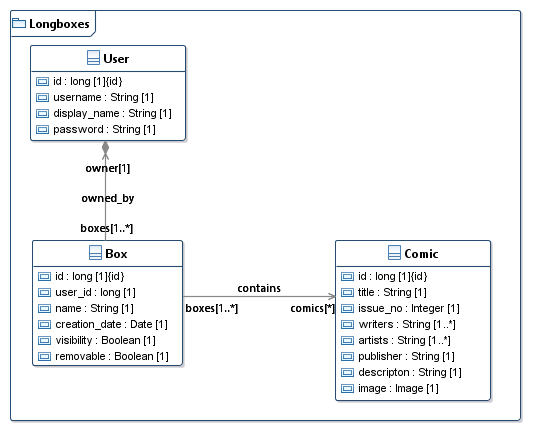
\includegraphics{UML_conceptual_design}
	\end{center}
	\caption{A UML class diagram of the conceptual design for the Longboxes application.}
	\label{fig:UML_conceptual_design}
\end{figure}


\subsection{Annotations}

The specification provided by the assessment document requires that a user of the application must have a user name, a screen name and a password. These are captured as attributes in the 'User' class. As users are provided with a default 'Unfiled' box, and as this is treated by various functions outlined in the specification as the user's default box, it simplifies the design of the application to require that this box exists.\\

Comic Boxes are defined in the specification as having an owner, a date on which they were created, a series of comics and a privacy setting. These are captured in the 'Box' class. The privacy setting has been interpreted as a boolean 'visibility' attribute rather than an enumeration as this simplifies the design and is sufficient to meet the requirement to display only 'Public' boxes to users other than the box owner. A visibility value of 'True' is interpreted as the box being 'Public' and a value of 'False' as the box being 'Private'. An extra attribute 'removable' has been attached to ensure that 'Unfiled' boxes cannot be removed.\\

Comics are defined by the specification and amendments on the module website to have a 400 by 300 pixel cover image (or 300 by 400 at the implementer's discretion), a title, an issue number, one or more writers, one or more artists, a publisher and a description. These are captured in the 'Comic' class.\\


\clearpage
\section{Transaction Map}

\begin{table}[h]
	\begin{threeparttable}
		\begin{tabular}{ p{0.5cm} p{10cm} p{1.4cm} p{1.4cm} }
			\hline
			& Transaction & Controller & Function \\
			\hline
			1a & Requirement removed after query on the module website & n/a & n/a \\
			1b & Search for a comic by title & main & search \\
			1c & Search for a comic by writer & main & search \\
			1d & Search for a comic by artist & main & search \\
			1e & Search for a comic by publisher & main & search \\
			\hline
			2a & Create a box & boxes & create \\
			2b & Remove a box & boxes & remove \\
			2c & Change a box's name & boxes & edit \\
			2d & Copy a comic to a box from a box owned by the user & comics & copy\tnote{1} \\
			2e & Change a box's visibility & boxes & edit \\
			2f & Copy a comic to one or more boxes from any box & comics & copy\tnote{2} \\
			2g & Remove a comic from a box owned by the user & comics & remove \\
			2h & View the contents of a box & boxes & box \\
			\hline
			3a & Create a comic & comics & create \\
			3b & Update a comic's details & comics & edit \\
			3c & View a comic's details & comics & comic \\
			3d & Delete a comic owned by the user & comics & remove\_ entirely \\
			\hline
			4a & On viewing the home page, present users with the five largest boxes and five newest boxes & main & index \\
			4b & On signing in, present users with their collection & main & user\tnote{3} \\
			4c & View public parts of other user's collections & main & user \\
			4d & View all comics in a collection at once & main & user\tnote{4} \\
			4e & Copy a comic to from another user's box & comics & copy\tnote{2} \\
			\hline
		\end{tabular}
		
		\begin{tablenotes}
			\item[1] handled by the 'copy' section
			\item[2] handled by the 'clone' section
			\item[3] this is treated as a special case of viewing user collections
			\item[4] handled by the 'view\_comics' section
		\end{tablenotes}
		
		\caption{The transactions the Longboxes application must provide, and the Web2Py controllers/functions in which they are implemented.}
		\label{tab:transaction_map}
	\end{threeparttable}
\end{table}
\clearpage


\section{Logical Design}

The assessment document specifies that each box may hold many comics, and clarifications on the module website allow comics to be in multiple boxes. This creates a many-to-many relationship between boxes and comics. To optimise database performance and simplify the implementation process this relationship has been resolved into two many-to-one relationships by the insertion of a mapping class ('Comic-Box Mapping') shown in \autoref{fig:UML_logical_design}. Each mapping links one box with one comic.

\begin{figure}[h]
	\begin{center}
		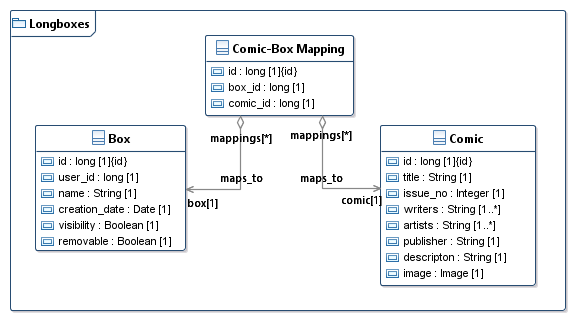
\includegraphics{UML_logical_design}
	\end{center}
	\caption{An abbreviated UML class diagram which introduces a mapping class between boxes and comics.}
	\label{fig:UML_logical_design}
\end{figure}


\subsection{Referential Integrity}

Boxes belong to specific users, and should be removed when their associated user is removed. This is a cascaded deletion, which is the default provided by Web2Py.\\

Comic-Box mappings link comics with boxes, but the boxes and comics involved in the relation do not belong to the relation and so should not be removed if a link is removed. However if a box or comic is deleted then any mappings involving that comic/box become invalid and should be removed. This is again the default functionality provided by Web2Py.
	

\chapter{User Interface Design Rationale}

\section{User Journey - Feedforward and Feedback}

\textbf{End Goals:} Edit a comic's image\\
\textbf{Journey Summary:} Load the site $\rightarrow$ Sign in $\rightarrow$ View the user's boxes $\rightarrow$ View a box's contents $\rightarrow$ View a comic $\rightarrow$ Upload a new image for the comic\\

When the site index page loads, the navigation bar should be identifiable as it is placed in a conventional position along the top of the screen, and as it contains a series of sections that are expected in a navigation bar (a home 'button', a series of navigation links and a sign in option). The 'Sign In' link is then in a standard position on the right of this bar. The link also changes colour when hovered over to further indicate that it is a hyperlink. After clicking on the 'Sign In' link the user is directed to the 'Sign In' page. This similarity in terms used indicates to the user that they have successfully reached the functionality that they intended to.

On loading the sign in form an 'active' effect appears around the first text box making it seem interactive, and a flashing cursor becomes visible to indicate that the field can be typed in. Once the user has entered their details, they should notice the differently coloured and slightly outset button. After clicking the 'Log In' button the user is directed to their box collection. The user should recognise the boxes as their own, and this demonstrates that they have signed in successfully.

The user's boxes are presented as a series of images with attached details. As the images are more vibrant than their surroundings they should attract the user's attention and on inspection appear interactive. If this fails, the user should instead notice that the first line of text under each comic is a hyperlink (as they are coloured hyperlink blue). Once the user clicks on one of these links they are directed to a page containing a view of the comics contained in the box. The image that the user clicked on to get to the box will be present in the top-right of the view confirming that the user has navigated to where they expected. A similar identification process to the one used to identify box links can be used to identify the comic links on the box page.

The full details for the selected comic will then be displayed. The user should notice that in the header section there are a series of hyperlinked icons. The purpose of these icons should be obvious as they depict objects the user is familiar with from the physical world. For example, clicking the 'pencil' icon allows the user to edit a comic.

When uploading a new image a validation check is performed to ensure that the image is the correct size. If there is an error an error message is displayed in a typical red error colour, and an error bar appears across the top of the page in case the user misses the error message. If the upload is successful then a preview of the image is shown.


\clearpage
\section{User Journey - Visual Layout}

\textbf{End Goal:} Read the description of a newly added comic (potentially as part of a search to find new comics)\\
\textbf{Journey Summary:} Load the site $\rightarrow$ View the newest box's contents $\rightarrow$ View the details of a comic in that box $\rightarrow$ Identify and read the comic's description\\

On loading the Longboxes site, the user is presented with a page with three distinct sections. The first of these is the site header, which has it's background and text colours inverted (compared to the rest of the page) to mark it as separate to the main content on the page. The second and third sections contain a series of box elements with each section using approximately 50\% of the remaining vertical space (indicating that they are of roughly the same importance).

The two sections are separated by whitespace to differentiate between the two categories, but the lack of a hard barrier between them (e.g. a line) indicates that they are still related to some extent (they both present a series of boxes).

These sections are then broken down into a series of elements. Each element has the same format, starting with a rectangular image followed by some text underneath. The section headings, the text beneath each image and the small box-like image at the bottom of the comic image together identify these elements as boxes.

The hierarchical structure of the page combined with a logical ordering of the newest comics (from newest to oldest, as suggested by the heading 'Newest Collections') allows the user to quickly identify that they are interested in the bottom-left-most box. The user can then click the box image, or if it's not obvious that the image can be clicked then the user can use the hyperlink on the box name. Either option will result in the user being directed to a page displaying the box's contents.

Once the user reaches the box page, their attention will likely be directed first to the centred heading section, and then to the graphical section below it. The graphical section here should seem different to the sections on the first page as the text attached to each image is to its right rather than below it, and consequently the flow of the elements is different.

This change in layout, combined with the absence of the small box images at the bottom of each image should cause the user to notice that although these images are similar to those on the index page, these images represent something else. Contextual clues such as the purpose of the site and the details provided should inform the user that these images represent comics.

After identifying that the images represent comics, the user can then click the comic image (or use the hyperlink if this isn't obvious) to navigate to the comic's details.

The user is then presented with a page in three sections: a heading section, an image section and a details section. The description is extra information about a comic and so is likely to be in the details section. The description is then set apart vertically from the other details, and should be distinguishable by the lack of a heading and (usually) the comparative length of the text block.


\end{document}